\htwo{OpenAPI}
\begin{figure}
    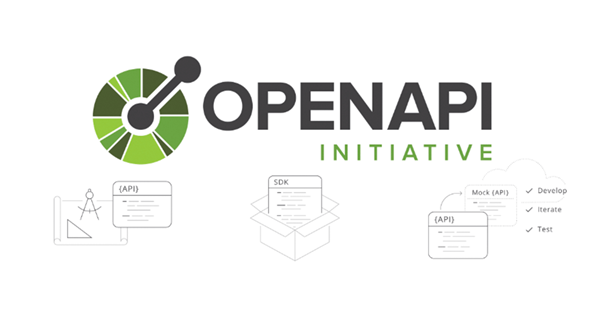
\includegraphics{media/OpenAPI/Logo.png}
    \centering
    \caption{Logo von OpenAPI}
\end{figure}

Die OpenAPI-Spezifikation ermöglicht es die Struktur einer REST-API so darzustellen, dass sie sowohl von Menschen als auch von Computern gelesen werden kann. Angefangen hat die OpenAPI-Spezifikation als Teil des Softwareprojekt "Swagger", einem Open-Source-Framework für HTTP-Webservices. Seit 2016 ist OpenAPI ein selbstständiges Projekt und wird von der OpenAPI-Initiative verwaltet. OpenAPI-Definitionen werden in einem Dokument abgespeichert. Geschrieben werden diese Dokumentationen dann entweder in JSON oder in YAML. Die Zelia-API wurde ebenfalls mithilfe von OpenAPI in YAML beschrieben. Wie ein OpenAPI-Dokument strukturiert ist, wird anhand der Zelia-API erläutert. Wichtig zu beachten ist bei der Verwendung von YAML die Einrückungen, die in dieser Sprache essenziell sind.

\yaml{code/OpenAPI/Description.yaml}{Beschreibung der OpenAPI-Version}

In der ersten Zeile wird die OpenAPI-Version angegeben. Die Version muss in jeder API-Spezifikation enthalten sein. Im "info"-Block werden Projektname und Informationen über den Autor beschrieben. Der "servers"-Block enthält Informationen zu der URL des Webservices. 

\yaml{code/OpenAPI/Rauminfo.yaml}{TODO: caption}

Der "paths"-Block ist das Herzstück des Dokuments und beschreibt die verschiedenen Pfade, die in der API definiert sind. Im oberen Teil des Blockes wird der Pfad und seine Aufgabe kurz zusammengefasst. Der Wert vom "operationId"-Key legt einen Namen für eine möglicherweise später genutzte Methode im Programmcode fest. Der "responses"-Block beinhaltet alle möglichen Antworten des Webservers. In dem gezeigten Beispiel gibt es für den "/api/room/"-Pfad zwei Antwortmöglichkeiten. Die erste Antwort ist eine reguläre Antwort mit HTTP-Statuscode 200. In dem dazugehörigen Block wird die Antwort genauer beschrieben. Der Wert des "type"-Keys gibt an, von welchem Typ der Inhalt der Antwort ist. Weiters kann man mithilfe des "x-examples"-Block eine mögliche Antwort darstellen. Diese dient nur zur Verständlichkeit. Der "500"-Block definiert die Antwort im Falle eines Internal Server Errors. Theoretisch könnten noch mehrere Statuscodes definiert werden, in diesem Fall werden jedoch nur zwei benötigt. Diese Vorgehensweise wird bei der Beschreibung der REST-API nun für jeden einzelnen Pfad angewendet. Das fertige Dokument soll die Beschreibung für jeden einzelnen Pfad beinhalten. In diesem Kapitel der Arbeit wird nicht jeder einzelne Pfad des Zelia-OpenAPI-Dokuments gezeigt.

\yaml{code/OpenAPI/ZeliaComponents.yaml}{TODO: caption}

Ein weiterer nützlicher Block in einem OpenAPI-Dokument ist der "components"-Block. Oft ist es der Fall, dass mehrere API-Operationen dieselben Parameter oder dieselbe Response-Struktur haben. Um eine Wiederholung von Code zu vermeiden, können im "components"-Block Typen definiert werden. Auf diese Typen kann dann an anderen Stellen des Dokuments zugegriffen werden. 

Zusammengefasst stehen in einem OpenAPI-Dokument Informationen über den Autor des Dokuments, URL des Webservices und Informationen über alle Pfade innerhalb einer REST-API. 

